\documentclass[tikz,14pt,fleqn]{article}
\usepackage{footnote}
\usepackage[bottom]{footmisc}
\makesavenoteenv{tabular}
\makesavenoteenv{table}

% Math
\usepackage[fleqn]{amsmath}
\usepackage{amssymb}
\usepackage{dsfont}
\usepackage{float}


% Make a dirtree
\usepackage{dirtree}
% Insert dummy text
\usepackage{lipsum}
% Allows to use caption*
\usepackage{caption}
% Scalable subfigures and subcaptions
\usepackage{subcaption} 
% H positioning
\usepackage{float}
% Wrap text around figures
\usepackage{wrapfig}
% Code syntax highlighting
\usepackage{minted}
% Plots
\usepackage{pgfplots}
% Allows to use custom enumerate items such as i), ii) iii)
\usepackage{enumitem}
% Draw diagrams and circuits
\usepackage{circuitikz}

% Define colors
\usepackage{xcolor}
\definecolor{ACCENT}{HTML}{E74C3C}
\definecolor{CODEBG}{HTML}{FAFAFA}
\definecolor{REFERENCES}{HTML}{E74C3C}
\definecolor{URL}{HTML}{E74C3C}
\definecolor{CITATION}{HTML}{E74C3C}
% Hyperlinks
\usepackage{hyperref}
\hypersetup{
    bookmarksopen=true,
    bookmarksopenlevel=0,
    hypertexnames=false,
    colorlinks=true,% Set to false to disable coloring links
    citecolor=CITATION,% The color of citations
    linkcolor=REFERENCES,% The color of references to document elements (sections, figures, etc)
    urlcolor=URL,% The color of hyperlinks (URLs)
    pdfstartview={FitV},
    unicode,
    breaklinks=true,
}
\setminted{fontsize=\small, framesep=2mm, tabsize=4}

% "Figure X" refs
\usepackage{cleveref}

% includegraphics
\usepackage{graphicx}

% Use icons
\usepackage{fontawesome}

\newcommand{\bmat}[1]{
   \ensuremath{
   \begin{bmatrix}
       #1
   \end{bmatrix}
}}

\newcommand\anonref[1]{\hyperref[#1]{\textsuperscript{\#}}}
\newcommand\exthref[2]{\href{#1}{\faicon{share-square-o} #2}}

%%%% LAYOUT %%%%

% Footnotes in tables
\usepackage{footnote}
\makesavenoteenv{tabular}
\makesavenoteenv{table}
\usepackage[bottom]{footmisc} % places footnotes always at page bottom

% Customize page layout
\usepackage{geometry}
\geometry{a4paper, margin=1in}

% Page headers and footers
\usepackage{fancyhdr}
\pagestyle{fancy}
\fancyhf{}
\setlength{\parindent}{0pt}
\setlength{\parskip}{0.5\baselineskip}%
% 



\usepackage[utf8]{inputenc}


%%%%%%%%%%%%%%%%%%%%%%%%%%%%
%% VARIABLES
\newcommand\namesurname{Albert Cerfeda (20-980-272)}
\newcommand\assignment{Assignment 1}

\newcommand\subject{Advanced Systems Lab}
\newcommand\documentdate{28.02.2024}

% Title content
%%%%%%%%%%%%%%%%%%%%%%%%%%%%
\rhead{\assignment}
\lhead{\namesurname}
%%%%%%%%%%%%%%%%%%%%%%%%%%%%

\rfoot{Page \thepage}


\begin{document}

\begin{titlepage}
   \begin{center}
       \vspace*{0.2cm}

       \textbf{\Large{\subject}}

       \vspace{0.5cm}
        \textbf{\assignment}\\[5mm]
        
            
       \vspace{0.4cm}

        \namesurname
        \begin{figure}[H]
            \centering
        \end{figure}
       \tableofcontents 

       \vspace*{\fill}
     
        
\includegraphics[width=0.3\textwidth]{fig/eth_logo_kurz_pos.eps}
       
        \documentdate \\ 
        Eidgenössische Technische Hochschule Zürich\\
        D-INFK Department\\
        Switzerland\\

   \end{center}
\end{titlepage}

\renewcommand{\thesubsubsection}{\alph{subsubsection})}
\setcounter{section}{1}
\setcounter{subsection}{0}

\subsection{(15 pts) Get to know your machine}

\subsubsection*{a) - d)}
Below you can see microarchitectural parameters of the laptop used to complete this Homework. \textbf{Note}: Apple is notoriously secretive about the detailed specifications of their devices, so the table has been filled on a best-effort basis.
\begin{table}[h!]
    \begin{tabular}{l|l}
     Processor manifacturer & TSMC\\
     \hline \hline Processor name & Apple M1 Pro (2021) \\ 
     \hline Serial number & KP9H9FY0KF\footnote{Serial number: The device serial number is indicated, since there is no apparent serial number for the processor itself provided by Apple.} \\
     \hline Microarchitecture & Firestorm/Icestorm\footnote{Firestorm/Icestorm: The microarchitecture of the Apple M1 Pro (2021) uses \textit{Firestorm} for its performance cores and \textit{Icestorm} for its efficiency cores [Source: \exthref{https://www.notebookcheck.net/Apple-M1-Pro-Processor-Benchmarks-and-Specs.579915.0.html}{notebookcheck.net}]}\\
     \hline CPU Base Frequency & 3.28 GHz (performance cores), 2.06 GHz (efficiency cores) \\
     \hline CPU Maximum Frequency & Not available \\ %TODO: CPU Maximum Frequency: find out
     \hline Support for Intel Turbo Boost or similar & No \\
    \end{tabular}
    \caption{Microarchitectural parameters}
\end{table}

\subsubsection*{e)}
\begin{wrapfigure}{l}{0.6\linewidth}
    \vspace*{-0.5cm}
    \begin{subfigure}{1\linewidth}
        \centering
        \inputminted[fontsize=\scriptsize, bgcolor=CODEBG]{C}{../ex1/fp_instruction_set.c}
        \caption{C code performing floating point division}
        \label{fig:fp_instruction_set_c}
    \end{subfigure}\\
    \begin{subfigure}{1\linewidth}
        \centering
        \inputminted[fontsize=\scriptsize, bgcolor=CODEBG]{asm}{../ex1/fp_instruction_set.s}
        \caption{\small Compiled assembly code, using \texttt{GCC} \\(Apple clang version 15.0.0) and \texttt{-O3} optimization level}
        \label{fig:fp_instruction_set_asm}
    \end{subfigure}
    % \vspace*{-2.5cm}
    \caption{Floating point division compilation}
\end{wrapfigure}
In \autoref{fig:fp_instruction_set_asm} we can see the assembly code generated by the \texttt{GCC} compiler for the C code shown in \autoref{fig:fp_instruction_set_c}.\\
Using \texttt{Apple clang}, the resulting compiled code utilizes the \texttt{FDIV} instruction for performing floating point division. While the instruction shares the same name as the one used in the x86 architecture, it is important to note that the underlying microarchitecture of the Apple M1 Pro is ARM-based, and the instruction set is \texttt{ARMv8.5-A}. Furthermore, SSE/SSE2 is not supported.
\\\\\\\\
\subsubsection*{f)}
The x86 floating point operations are included in the standard x86 instruction set architecture while SSE/SSE2 is an extension of the x86 instruction set. Both operate on special dedicated registers, with the difference that the x87 FPU have a higher precision, while the SIMD registers are 128 bits, allowing to perform arithmetic operations on multiple floating points in parallel.


\subsubsection*{g)}
For the following exercises the \exthref{https://dougallj.github.io/applecpu/firestorm.html}{Dougall Johnson's documentation} about the Firestorm architecture has been used. The article mentions that Firestorm has a pipeline width of 8 instructions per cycle, and 4 SIMD ports each of which can execute both floating-point and SIMD instructions. So the maximum would be 4 floating-point operations per cycle.
\subsubsection*{h)}
The article does not seem to make a difference between single and double precision, so the latency for addition is 3 and throughput is is 4, for both single-precision and double precision.
\subsubsection*{i)}
% TODO: Latency and througput for single precision reciprocal square root

\subsubsection*{j)}
The latency for FP division is 10 and throughput is 1.


\subsection{(20 pts) LU Factorization}
\subsubsection{} % a)
% \begin{figure}[h!]
%     \vspace*{-0.5cm}
%     \inputminted[fontsize=\scriptsize, linenos, bgcolor=CODEBG, firstline=57, lastline=70]{C}{../ex2/lu.c}
%     \caption{\texttt{compute} function inside \texttt{lu.c}}
% \end{figure}

\subsubsection{} % b)
The \texttt{compute} function performs $n^2$ FP divisions, $n^3$ FP multiplications and $n^3$ FP subtractions, for a total of $n^2 + 2n^3$ floating point operations. \textbf{Note:} Subtractions are reported since they are typically implemented using additions, due to 2s complement arithmetic.
% TODO: Subtractions count as additions due to 2s complement arithmetic ?
\subsubsection{} % c)
% Make a PGF plot that imports data points from a file
\begin{figure}[H]
    \vspace*{-0.7cm}
    % Include a PDF using the graphicx package
    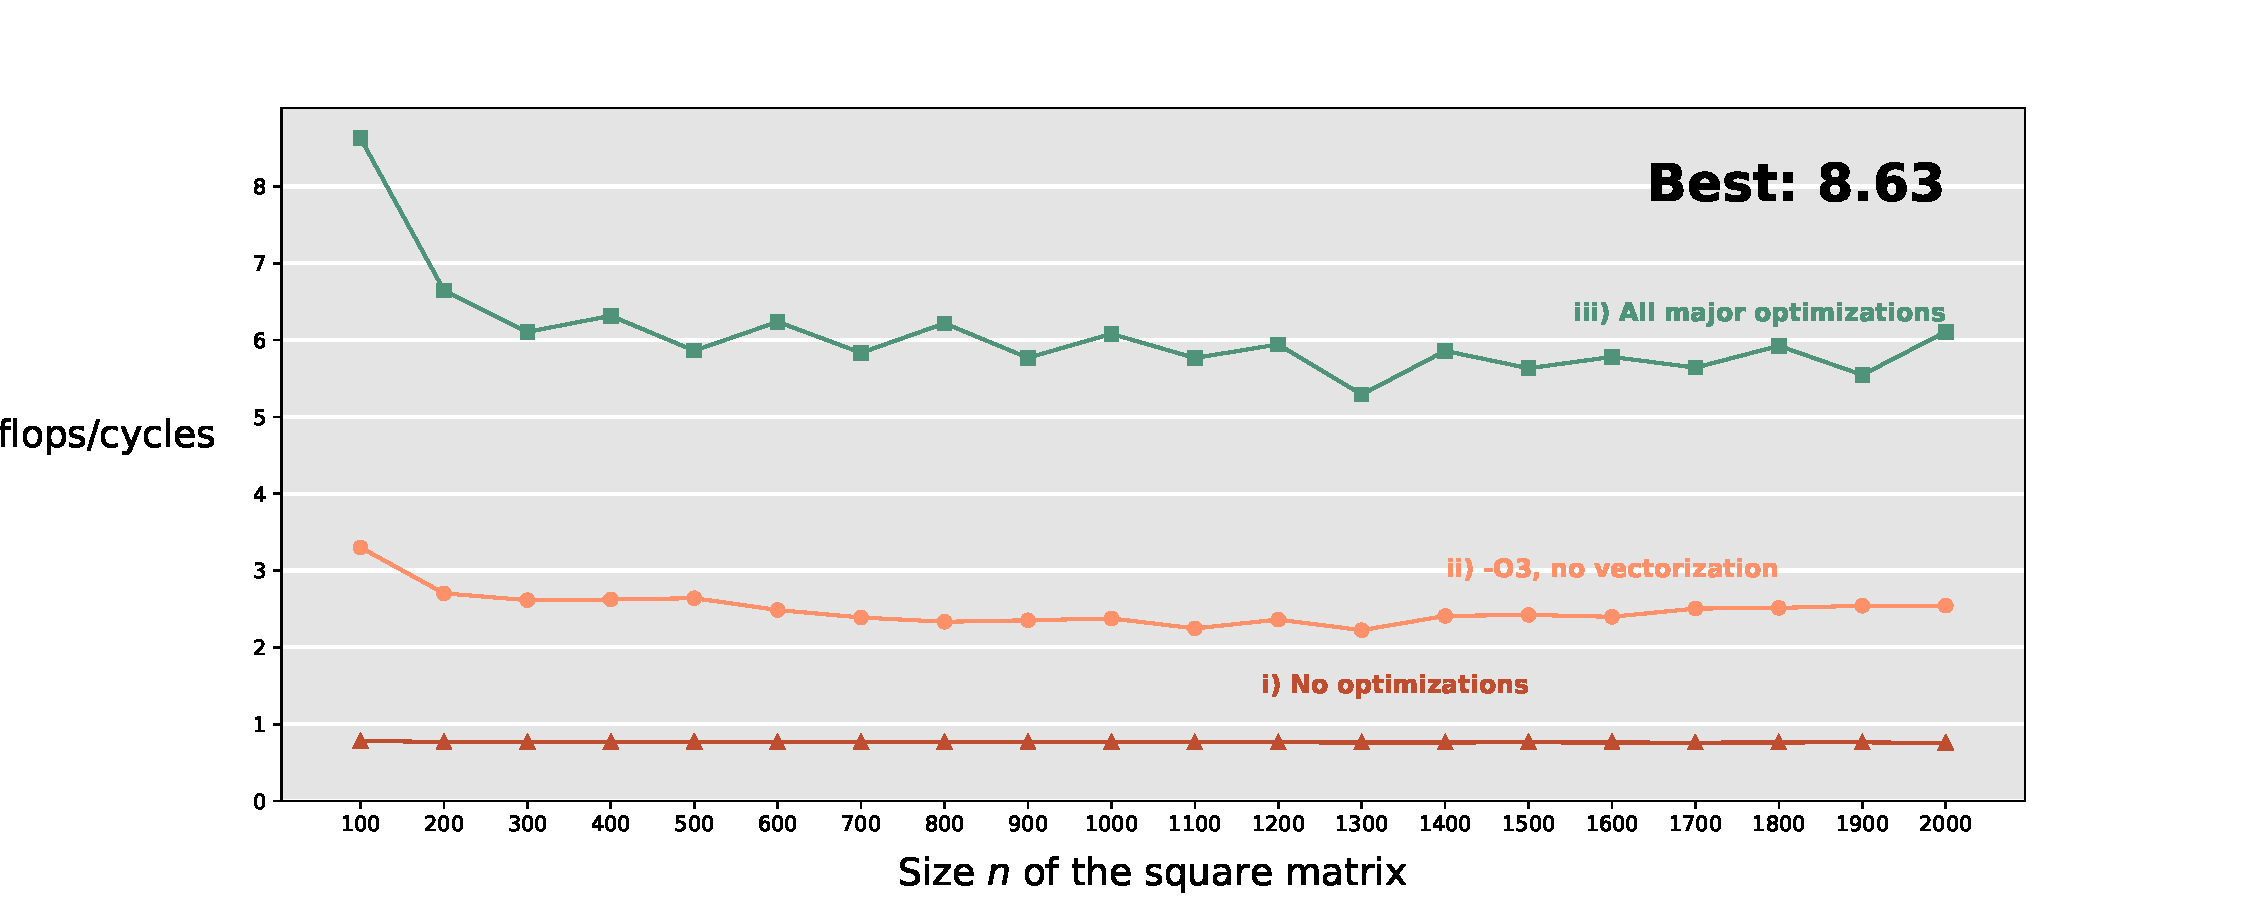
\includegraphics[width=\linewidth]{../out/ex2c.pdf}
    \caption{flops/cycle performance of the \texttt{compute} function compiled with different optimization flags}
\end{figure}


\subsubsection{} % d)
\begin{enumerate}
    \item No optimizations: The code is neither optimized nor vectorized. The performance is the worst and flat across the line.
    \item Optimized, but no vectorization: The compiler performs some optimizations resulting in a performance improvement, but no vectorization is performed.
    \item All major optimizations: The compiler both performs optimizations and vectories the code, resulting in the best performance. We also notice how for the matrix sizes we tested, the performance does not seem to vary greatly. The peak performance recorded is around \input{../out/ex2c_best.txt} flops/cycles.
\end{enumerate}

\subsection{(25 pts) Performance analysis and bounds}
\subsubsection{} % a)

\subsubsection{} % b)

\subsubsection{} % c)

\subsubsection{} % d)


\subsection{(25 pts) Basic optimization}
\subsubsection{} % a)
\begin{figure}[h!]
    \begin{subfigure}{1\linewidth}
        \inputminted[fontsize=\scriptsize, bgcolor=CODEBG, firstline=62, lastline=68]{C}{../ex4/lu4.c}
    \end{subfigure}\\
    \begin{subfigure}{1\linewidth}
        \inputminted[fontsize=\scriptsize, bgcolor=CODEBG, firstline=62, lastline=82]{C}{../ex4/lu4_optimized.c}
    \end{subfigure}
    \caption{Unoptimized and optimized \texttt{comp} functions}
    \label{fig:4.comp_functions}
\end{figure}
\begin{figure}
    \vspace*{-0.7cm}
    % Include a PDF using the graphicx package
    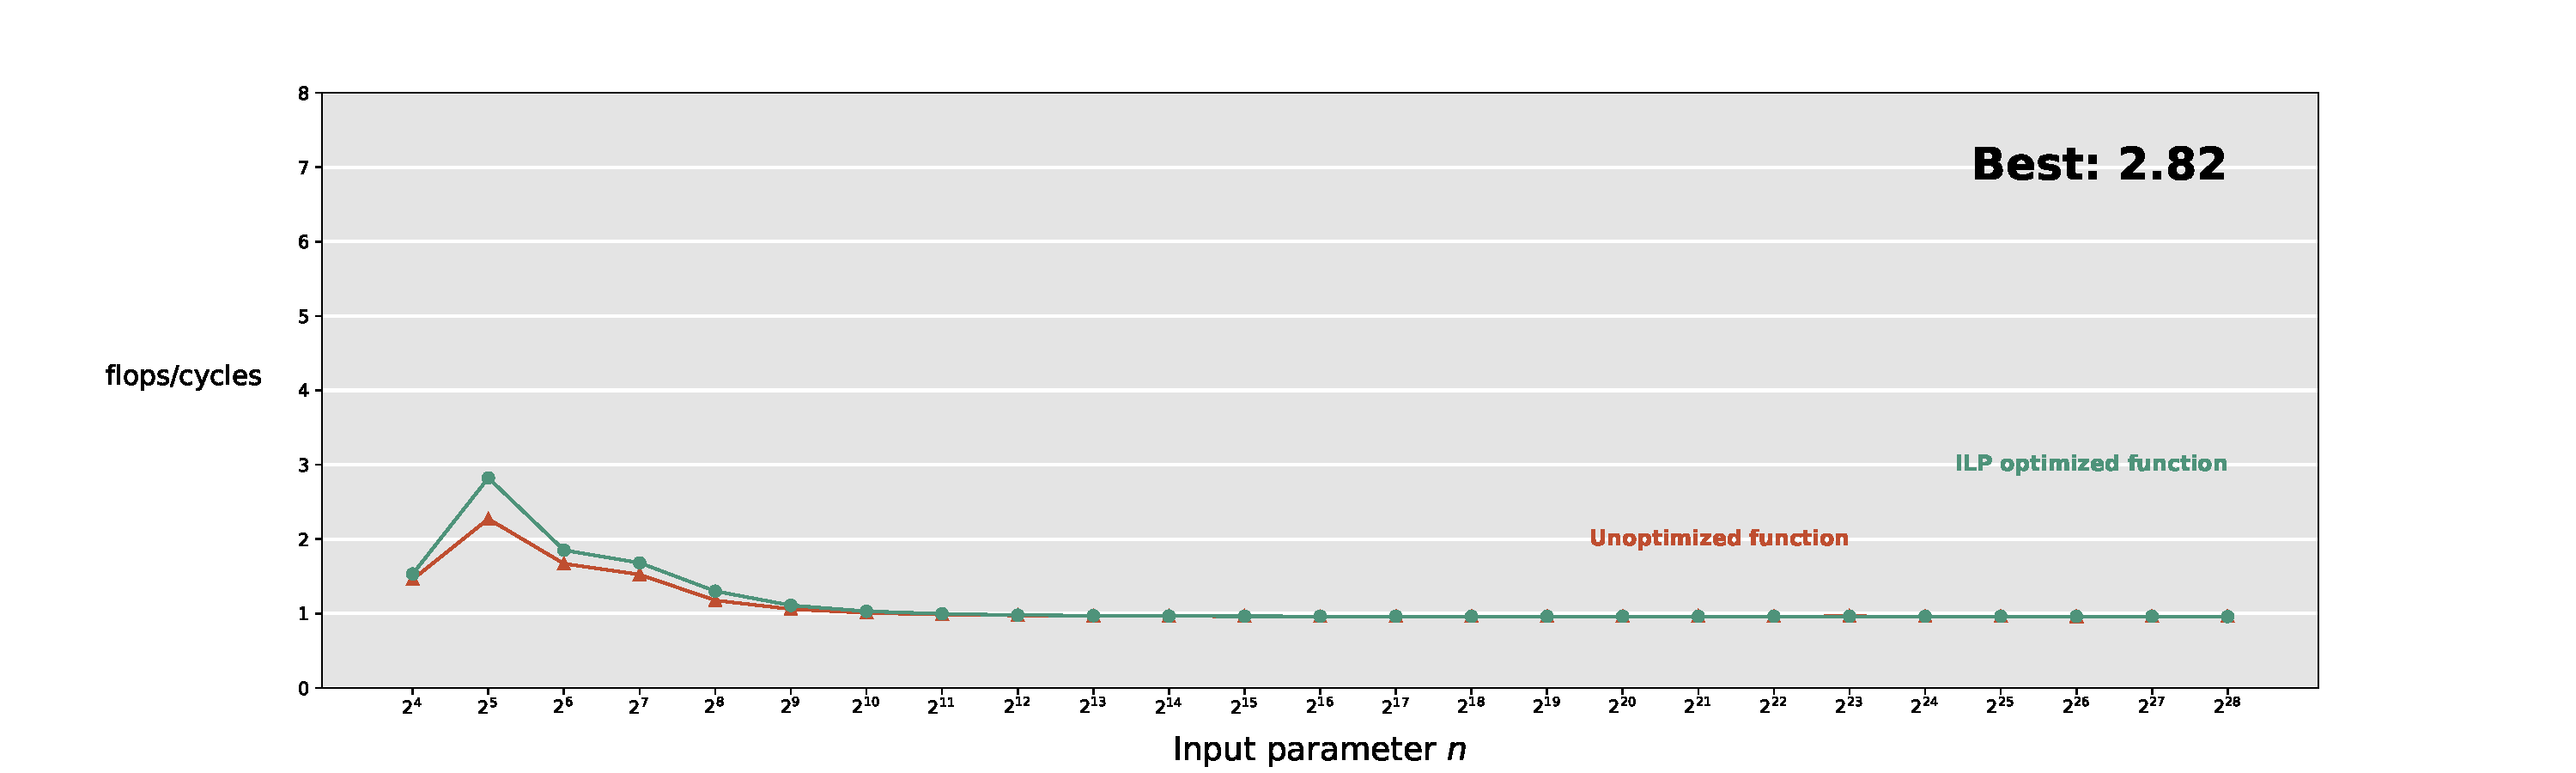
\includegraphics[width=\linewidth]{../out/ex4.pdf}
    \caption{flops/cycle performance of the \texttt{comp} functions}
    \label{fig:4.comp_functions_plot}
\end{figure}
\subsubsection{} % b)
% TODO: Is it just enough to look at the plot and see what the flops/cycles are to state an upper bound ?
\subsubsection{} % c)

% \end{figure}
\subsubsection{} % d)
\autoref{fig:4.comp_functions} shows a comparison between the unoptimzied \texttt{comp} function and its optimized counterpart. In order to improve ILP I perfomed 3x loop unrolling and introduced accumulators for reducing memory accesses to the array \texttt{z}. Initially I implemented 4x loop unrolling, but the performance overhead became noticeable so I resorted to a lower 3x loop unrolling.

When running the optimized function on Code Expert, we obtain a $2.73$ speedup, but as you can see from the plot in \autoref{fig:4.comp_functions_plot}, when compiling and benchmarking on my Macbook M1 machine, there isn't any performance improvement over the unoptimized version. This is due to the \texttt{Apple Clang} compiler and that M1 is a different architecture to the one used to run the benchmarks on Code Expert. The best performance recorded on my machine is around \input{../out/ex4_best.txt} flops/cycles.

% \subsubsection{} % e)


\subsection{(10 pts) ILP analysis}
\subsubsection{} % a)
\begin{wrapfigure}{l}{0.5\linewidth}
    \centering
    \vspace*{-0.7cm}
    \begin{subfigure}{\linewidth}
        \inputminted[fontsize=\scriptsize, linenos, bgcolor=CODEBG]{C}{../ex5/artcomp.c}
    \end{subfigure}
\end{wrapfigure}

\subsubsection{} % b)


% \subsubsection{}
% \includegraphics[width=0.9\linewidth]{fig/2a.png}

% \subsubsection{}
% \includegraphics[width=0.9\linewidth]{fig/2b.png}


% \subsection{Task 3}
% \subsubsection{}
% \includegraphics[width=0.9\linewidth]{fig/3a.png}

% \subsubsection{}
% \includegraphics[width=0.9\linewidth]{fig/3b.png}

% \subsubsection{}
% \includegraphics[width=0.9\linewidth]{fig/3c.png}

% \subsubsection{}
% \includegraphics[width=0.9\linewidth]{fig/3d.png}

\end{document}
